%%This is a very basic article template.
%%There is just one section and two subsections.
\documentclass{article}
\usepackage[latin1]{inputenc} %coding of writteninput %latin1 allows for Umlaute
\usepackage[T1]{fontenc}%vectorized fonts (cm-super package)
\usepackage[german]{babel}%some specifics of the german language
\usepackage{amsfonts, amsmath, amsthm, amssymb, mathabx, paralist}
 \setlength{\parindent}{0em} 
  \usepackage{listings}
\usepackage{geometry}
  \geometry{a4paper, top=25mm, left=20mm, right=15mm, bottom=20mm, headsep=10mm, footskip=12mm}
 \usepackage{rotating} 
 %Decisiontree
 \usepackage{tikz,forest}
\usetikzlibrary{arrows.meta}
  
\usepackage{graphicx} 

\usepackage{verbatim}%f�r txt datei

\usepackage{color} %red, green, blue, yellow, cyan, magenta, black, white
\definecolor{mygreen}{RGB}{28,172,0} % color values Red, Green, Blue
\definecolor{mylilas}{RGB}{170,55,241}
\usepackage{pdfpages}
\usepackage[section]{placeins}
\begin{document}
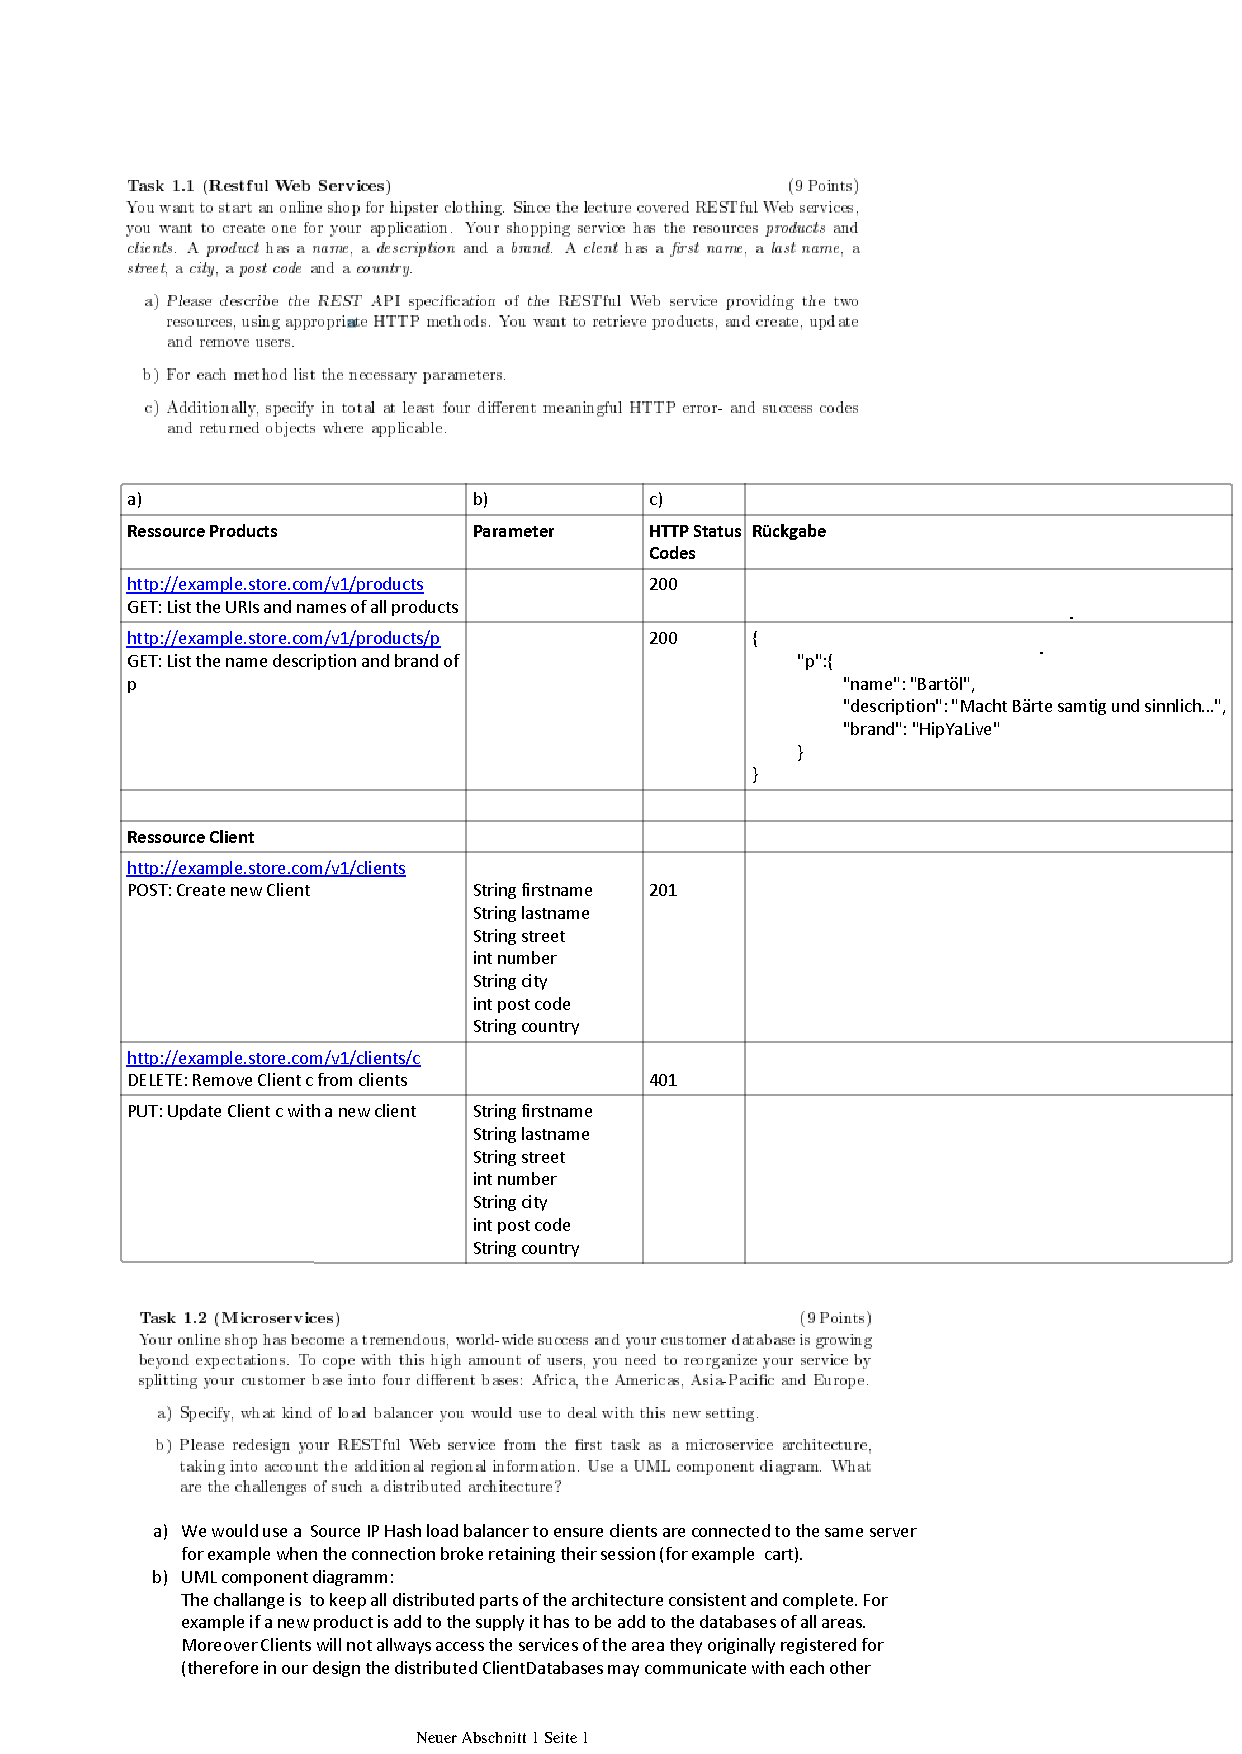
\includepdf[pages=-]{Blatt1.pdf}

\section*{Task 1.3 b)}
Like in the lecture visualized on the http level happen the following steps:
\begin{enumerate}
\item The application requests authorization to access service resources from
the user\\ 
\item If the user authorized the request, the application receives an
authorization grant\\
\item The application requests an access token from the
authorization server (API) by presenting authentication of its own identity, and the authorization grant
\item If the application identity is authenticated and the authorization grant
is valid, the authorization server (API) issues an access token to the
application. Authorization is complete.\\
\item The application requests the resource from the resource server (API) and
presents the access token for authentication\\
\item If the access token is valid, the resource server (API) serves the
resource to the application
\end{enumerate}
(https://www.digitalocean.com/community/tutorials/an-introduction-to-oauth-2)


\includepdf[pages=119]{SocialComputing-Infrastructures.pdf}

\section*{Task 1.3 c)}
If an attacker has acces to the network he can eavesdrop on the traffic and gain
acces. Creating tokens and shared-secrets that are long, random and resistant
to eavesdrop can help to avoid this.

Also it is possible, that the secrets aren't stored safety. Solution: The
secrets can be isolated and stored in a database or file-system with proper
access control, file permission, physical security, and even database or disk
encryption.


\end{document}
